\chapter{Diagnostic du public et choix du thème}
\section{Pourquoi interroger les stagiaires ?}

Le questionnaire du commanditaire nous a donné un premier cadre, mais il ne suffisait pas pour choisir un thème. Les risques cités concernaient l’établissement de manière générale et ne prouvaient pas que les stagiaires plombiers avaient les mêmes besoins.

Nous avons donc créé un questionnaire anonyme de trente questions destiné directement au groupe. Il abordait la situation de déplacement, la vitesse, le téléphone et les distracteurs, l’alcool, les stupéfiants, les médicaments, la ceinture et une dernière partie consacrée à la perception globale et aux attentes.

Les questions avaient trois objectifs simples : vérifier certaines connaissances, repérer des comportements déclarés et identifier des représentations pouvant influencer une décision. Plusieurs mises en situation ont été adaptées au métier de plombier : retard sur un chantier, appel d’un client, recherche d’adresse ou déplacement en véhicule utilitaire.

Le questionnaire a été transmis à Mme LIÉGEOIS le 26 octobre 2026. Après une relance le 29 octobre, nous avons reçu treize questionnaires exploitables. Les réponses sont anonymes et utilisées uniquement de manière collective.

\section{Méthode de lecture des réponses}

Pour l’analyse, j’ai séparé deux catégories :

— les connaissances et perceptions : réponse fausse, incertitude ou représentation pouvant conduire à sous-estimer un risque ;

— les comportements et situations à risque : comportement déclaré ou décision choisie dans une mise en situation.

Cette distinction est importante : une mauvaise réponse ne prouve pas un comportement dangereux, et un comportement déclaré ne permet pas d’affirmer qu’une infraction a été réellement commise.

Pour le graphique de synthèse, la partie H du questionnaire n’est pas utilisée dans le calcul car elle porte surtout sur les attentes et les thèmes que les stagiaires souhaitent aborder.

\section{Profil de déplacement du groupe}

Parmi les 13 répondants :

— 11/13 déclarent posséder le permis B ;

— 2/13 ne le possèdent pas ;

— 4/13 conduisent tous les jours ;

— 2/13 plusieurs fois par semaine ;

— 4/13 occasionnellement ;

— 3/13 ne conduisent jamais.

Le groupe est donc assez hétérogène. Je dois proposer une sensibilisation compréhensible aussi bien par les conducteurs réguliers que par les non-conducteurs ou futurs conducteurs.

\section{Deux besoins ressortent nettement}

La comparaison des six thèmes montre deux résultats principaux.

\begin{figure}[H]\centering
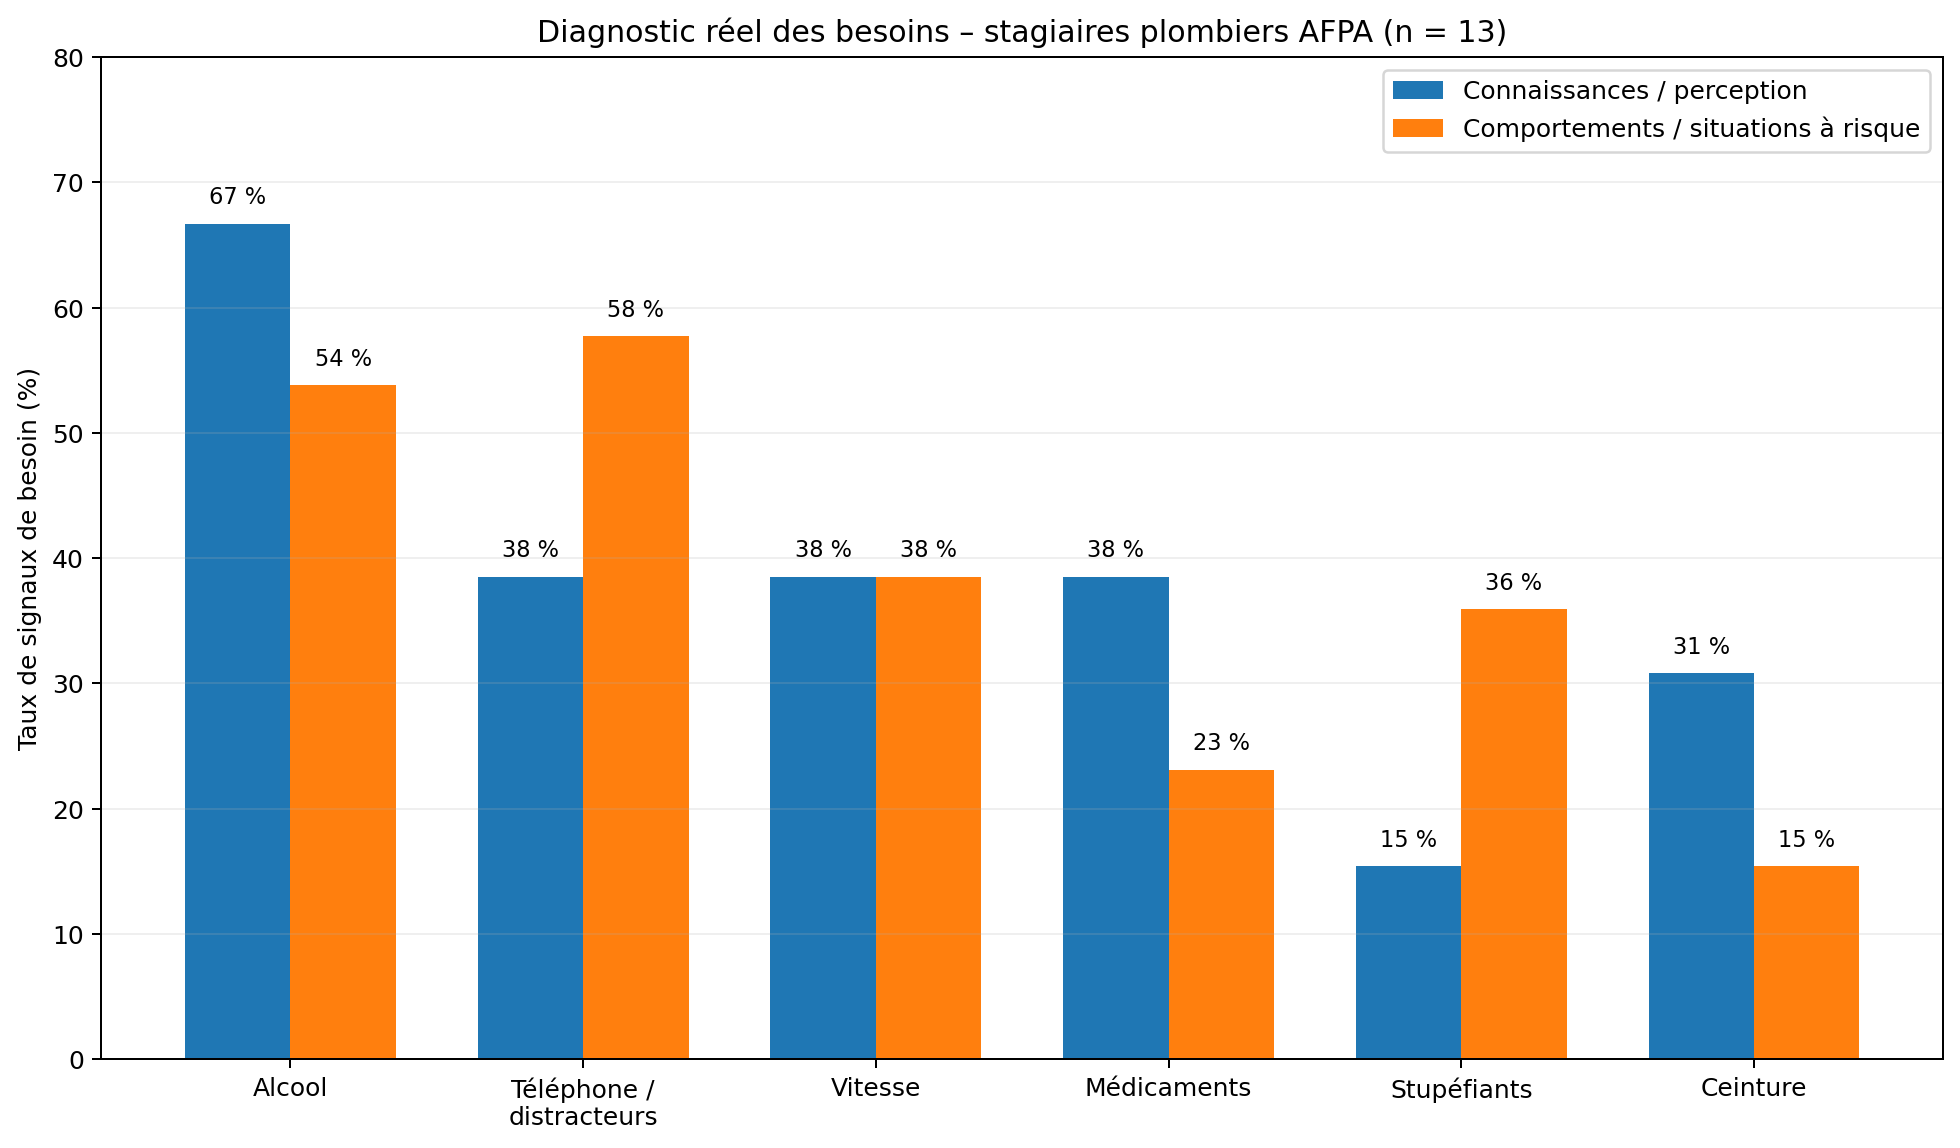
\includegraphics[width=0.92\textwidth]{images/diagnostic_afpa_13_repondants.png}
\caption{Signaux de besoin par thème pour les 13 répondants.}
\end{figure}

\begin{table}[H]
\centering\small
\caption{Lecture synthétique des réponses (n = 13)}
\begin{tabularx}{\textwidth}{@{}Xcc@{}}
\toprule
\rowcolor{bleuECSR}\textcolor{white}{\textbf{Thème}} & \textcolor{white}{\textbf{Connaissances / perception}} & \textcolor{white}{\textbf{Comportements / situations à risque}} \\
\midrule
Alcool & 69,23\,\% (9/13) & 53,85\,\% (7/13) \\
Téléphone / distracteurs & 38,46\,\% (5/13) & 61,54\,\% (8/13) \\
Vitesse & 38,46\,\% (5/13) & 38,46\,\% (5/13) \\
Médicaments & 38,46\,\% (5/13) & 23,08\,\% (3/13) \\
Stupéfiants & 15,38\,\% (2/13) & 38,46\,\% (5/13) \\
Ceinture de sécurité & 30,77\,\% (4/13) & 15,38\,\% (2/13) \\
\bottomrule
\end{tabularx}
\end{table}


\subsection{Alcool : surtout un besoin de connaissances et de perception}

L’alcool obtient le niveau le plus élevé dans la catégorie connaissances / perception : 69,23 \% (9/13). Le volet comportements / situations à risque atteint 53,85 \% (7/13).

Cela montre que l’alcool mérite une action de sensibilisation, notamment sur les effets, l’élimination et la confiance accordée à son propre ressenti. Comme nous travaillons en binôme, l’analyse détaillée de ce thème et sa réponse pédagogique sont développées par ma collègue Manane SADIK.

\subsection{Téléphone et distracteurs : surtout un besoin comportemental}

Pour le téléphone et les distracteurs, le résultat est différent : 38,46 \% (5/13) pour les connaissances et perceptions, mais 61,54 \% (8/13) pour les comportements et situations à risque. C’est le niveau comportemental le plus élevé des six thèmes.

Deux réponses m’ont particulièrement intéressé : 11/13 stagiaires savent qu’un dispositif mains libres ne supprime pas complètement le risque de distraction, mais 8/13 déclarent consulter une notification ou un message au volant au moins occasionnellement.

Ce décalage est important pour moi : connaître le danger ne suffit pas toujours à adopter la bonne décision. Dans le métier de plombier, cette situation peut se retrouver lors d’un appel client, d’un message du responsable, d’une recherche d’adresse ou d’un retard sur un chantier.
